\documentclass[ 11pt, a4paper, titlepage, DIV14, openright, BCOR8mm, headsepline]{scrreprt}
\usepackage[latin1]{inputenc}
\usepackage{graphicx}
\usepackage{caption}
\usepackage{subcaption}
\usepackage{epsfig}
\usepackage{pdfpages}
\usepackage{booktabs}
\usepackage{tabularx}
\usepackage{listings}
\lstset{basicstyle=\footnotesize\ttfamily,breaklines=true}
\usepackage{courier}
%\newcolumntype{C}[1]{>{\centering\arraybackslash}p{#1}}
%\newcolumntype{R}[1]{>{\raggedleft\arraybackslash}p{#1}}
\newcolumntype{C}{>{\centering\arraybackslash}X}
\usepackage{multicol}
\usepackage{multirow}
\usepackage{amsmath}
\usepackage{amssymb}
%\parindent 0pt
\bibliographystyle{unsrt}
\pagestyle{headings}
\usepackage[british,ngerman]{babel}
\usepackage{scrpage2}
\usepackage{perpage}
\MakePerPage{footnote}

\addtokomafont{caption}{\small}
\addtokomafont{captionlabel}{\bfseries}
%\addtokomafont{section}{\huge}
%\addtokomafont{subsection}{\Large}
%\addtokomafont{subsubsection}{\large}
\setkomafont{paragraph}{\normalfont\itshape}

\setcapindent{0mm}
\usepackage[colorlinks=false, pdfborder={0 0 0}]{hyperref}
\usepackage{url}
\usepackage{siunitx}

\sisetup{
	exponent-product = \cdot,
	range-units = brackets,
	range-phrase = -,
	per-mode = symbol}
\DeclareSIUnit[number-unit-product = {}]\c{$c$}

\pdfsuppresswarningpagegroup=1

\usepackage{draftwatermark}
\SetWatermarkScale{6}

\providecommand{\href}[2]{#2}   %generates the href macro if needed

\begin{document}

\graphicspath{{figures/}}

\subject{
\includegraphics[width=0.45\textwidth]{Logo}}
\title{\Huge{Getting Started}}
\subtitle{Version 1.30}
\author{Author:\\
		Patrick Eckert}
\date{}
\publishers{
		
\includegraphics[height=2cm]{LogoKIP}
		\hfill
		
\includegraphics[height=2cm]{LogoUniHD}
}

\maketitle


\textwidth		15.5cm
\textheight		23.0cm
\oddsidemargin	0.cm
\topmargin		0.cm

\pagenumbering{roman}

\selectlanguage{british}
\tableofcontents

\thispagestyle{plain}
\pagenumbering{arabic}

%======= Introduction =======%

\chapter{Introduction}

\paragraph{What can the simulation do for you?}\mbox{}\\

The simulation models the response (signal waveform and charge) of a SiPM to an arbitrary light pulse.
In order to model a specific SiPM, you have to provide a set of basic parameters for the simulation input.
For a precise simulating of the response, the input parameters have to be carefully measured!

\paragraph{What can the simulation NOT do?}\mbox{}\\

The simulation does not simulate the avalanche process itself and therefore cannot predict the basic parameters (e.g.\ PDE, gain, dark-rate, single pixel waveform,\dots) and their voltage and temperature dependence. This would require significantly more simulation effort and depends on the details of the doping structure which is typically not accessible.
In the GosSiP simulation the avalanche process is parameterised by the basic SiPM parameters, which can easily be measured (or taken from the data sheet).

\paragraph{What are typical application?}

\begin{itemize}
	\item Quickly compare different sensors for a specific application.
	\item Simulate the performance of a detector system using SiPMs (e.g.\ SiPM + scintillator).
	\item Analyse which SiPM parameters / noise sources limit the performance for your application.
\end{itemize}


%======= Installation =======%

\chapter{Installation}

\section{Linux, Mac}

\begin{itemize}
	\item{Requirements:}\\
		cmake, ROOT (\url{https://root.cern.ch/})
	
	\item{Download GosSiP source code from:}\\
		\url{http://www.kip.uni-heidelberg.de/hep-detektoren/gossip/versions}
		
	\item{Unzip files:}
	\begin{lstlisting}[language=bash]
$ unzip GosSiP\_Vx.xx.zip
$ cd GosSiP\_Vx.xx.zip
	\end{lstlisting}
		
	\item{Create build directory:}
	\begin{lstlisting}[language=bash]
$ mkdir build
$ cd build
	\end{lstlisting}
	
	\item{Run cmake:}
	\begin{lstlisting}[language=bash]
$ cmake
$ make
$ sudo make install
	\end{lstlisting}
		
	\item{You're ready to go:}
	\begin{lstlisting}[language=bash,belowskip=0em]
$ gossip
	\end{lstlisting}
	or
	\begin{lstlisting}[language=bash]
$ gossip 'your_sipm_parameter_file'
	\end{lstlisting}
\end{itemize}

\section{Windows}

You need to install Cygwin (\url{https://www.cygwin.com/}) to emulate a Unix shell.
Follow the Linux installation instructions using the Cygwin terminal.

	
%======= Simulation Principle =======%

\chapter{Simulation Principle}

\begin{figure}[h]
	\centering
	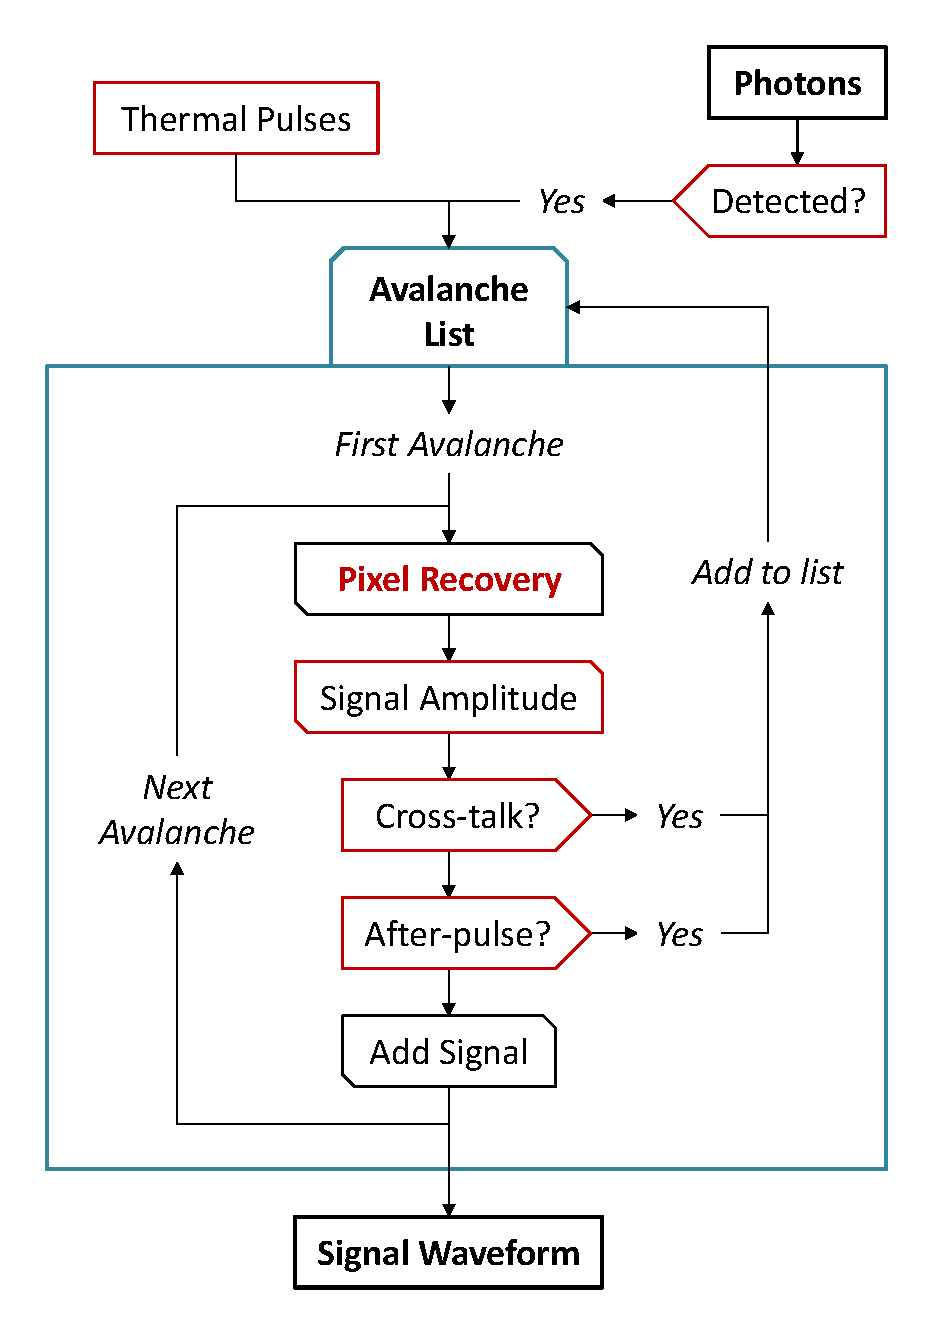
\includegraphics[width=0.75\textwidth]{SimulationFlow}
\end{figure}


%======= Input Parameters =======%

\chapter{Input Parameters}
\section{SiPM}

\begin{figure}[h!]
	%	\centering
	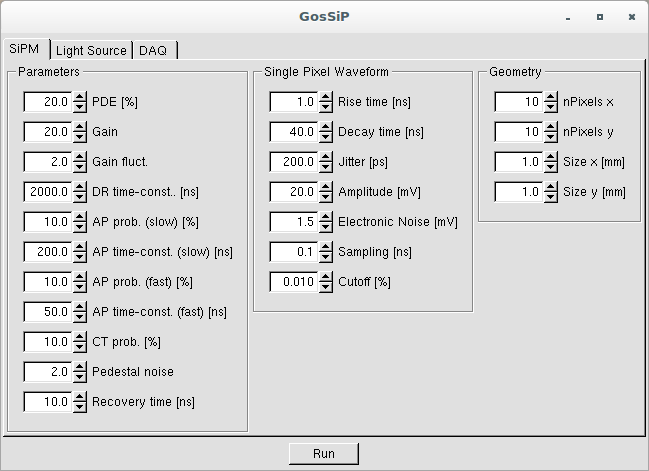
\includegraphics[height=0.25\textheight]{GUI1.png}
\end{figure}

All parameters are members of the sipmMC class.

\subsection*{Parameters}

\begin{description}
	\item[PDE] \textcolor{blue}{\textbf{(PDE)}}\\
		Photon detection efficiency (not including cross-talk and after-pulses).
	\item[Gain] \textcolor{blue}{\textbf{(gain)}}\\
		Gain in arbitrary units.
	\item[Gain fluct ] \textcolor{blue}{\textbf{(END)}}\\
		Gain fluctuations (same units as gain)
	\item[DR time-const] \textcolor{blue}{\textbf{(tau\_dr)}}\\
		Time constant of primary dark-counts, i.e.\ generated by thermal excitation or tunneling, excluding after-pulses.
	\item[AP prob (slow)] \textcolor{blue}{\textbf{(Pap\_s)}}\\
		Probability to trigger an after-pulse (slow component).
	\item[AP time-const (slow)] \textcolor{blue}{\textbf{(tau\_ap\_s)}}\\
		Characteristic time constant for after-pulses (slow component).
	\item[AP prob (fast)] \textcolor{blue}{\textbf{(Pap\_f)}}\\
		Probability to trigger an after-pulse (fast component).
	\item[AP time-const (fast)] \textcolor{blue}{\textbf{(tau\_ap\_s)}}\\
		Characteristic time constant for after-pulses (fast component).
	\item[CT prob] \textcolor{blue}{\textbf{(Pxt)}}\\
		Probability to trigger optical cross-talk.
	\item[Pedestal noise] \textcolor{blue}{\textbf{(EN)}}\\
		RMS width of the pedestal (same units as gain) (does only affect signal charge - not waveform).
	\item[Recovery time] \textcolor{blue}{\textbf{(tau\_recovery)}}\\
		Pixel recovery time.
\end{description}


\subsection*{Single Pixel Waveform}

\begin{description}
	\item[Rise time] \textcolor{blue}{\textbf{(SetPulseShape(double,double))}}\\
		Signal rise time - time constant of double exponential function.
	\item[Decay time] \textcolor{blue}{\textbf{(SetPulseShape(double,double))}}\\
		Signal decay time - time constant of double exponential function.
	\item[Jitter] \textcolor{blue}{\textbf{(jitter)}}\\
		Single pixel jitter.
	\item[Amplitude] \textcolor{blue}{\textbf{(signalAmp)}}\\
		Single pixel amplitude.
	\item[Electronic Noise] \textcolor{blue}{\textbf{(noiseRMS)}}\\
		Electronic noise (does only affect signal waveform - not charge).
	\item[Sampling] \textcolor{blue}{\textbf{(SetSampling(double))}}\\
		Sampling interval of waveform.
	\item[Cutoff] \textcolor{blue}{\textbf{(SetCutoff(double))}}\\
		The single pixel waveform is cut-off when the falling edge falls below a certain value. This \textit{cutoff} value is given in \% of the peak amplitude.
\end{description}

\subsection*{Geometry}

\begin{description}
	\item[nPixels x] \textcolor{blue}{\textbf{(NpixX)}}\\
		Number of pixels in x direction.
	\item[nPixels y] \textcolor{blue}{\textbf{(NpixY)}}\\
		Number of pixels in y direction.
	\item[Size x] \textcolor{blue}{\textbf{(xSipm)}}\\
		Size in x direction.
	\item[Size y] \textcolor{blue}{\textbf{(ySipm)}}\\
		Size in y direction.
\end{description}

\section{Light Source}

\begin{figure}[h!]
	%	\centering
	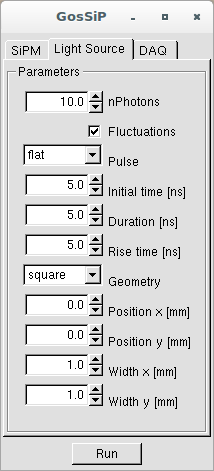
\includegraphics[height=0.25\textheight]{GUI2.png}
\end{figure}

All parameters are members of the LightSource class.

\begin{description}
	\item[nPhotons] \textcolor{blue}{\textbf{(SetNgamma(int))}}\\
		Mean number of photons in the light pulse.
	\item[Fluctuations] \textcolor{blue}{\textbf{(SetFluctuation(bool))}}\\
		Enables / disables fluctuations (Gaus/Poisson) in the number of photons.
	\item[Pulse] \textcolor{blue}{\textbf{(SetPulse(string))}}\\
		Time distribution of the photons (\textit{flat}: flat distribution, \textit{gaus}: gaussian distribution, \textit{exp}: exponentially decaying distribution, \textit{exp2}: double exponential distribution).
	\item[Initial time] \textcolor{blue}{\textbf{(SetTime(double))}}\\
		Starting time of the light pulse.
	\item[Duration] \textcolor{blue}{\textbf{(SetTimeWidth(double))}}\\
		Duration of the light pulse (\textit{flat}: duration, \textit{gaus}: sigma, \textit{exp}: decay time constant, \textit{exp2}: decay time constant).
	\item[Rise time] \textcolor{blue}{\textbf{(SetRiseTime(double))}}\\
		Rise time of the light pulse (only for \textit{exp2}!).
	\item[Geometry] \textcolor{blue}{\textbf{(SetShape(string))}}\\
		Spatial distribution of the photons (\textit{square}, \textit{elliptic}).
	\item[Position x] \textcolor{blue}{\textbf{(SetXY(double,double))}}\\
		Position in x direction.
	\item[Position y] \textcolor{blue}{\textbf{(SetXY(double,double))}}\\
		Position in y direction.
	\item[Width x] \textcolor{blue}{\textbf{(SetXYWidth(double,double))}}\\
		Width in x direction.
	\item[Width y] \textcolor{blue}{\textbf{(SetXYWidth(double,double))}}\\
		Width in y direction.
\end{description}


\section{DAQ}

\begin{figure}[h!]
	%	\centering
	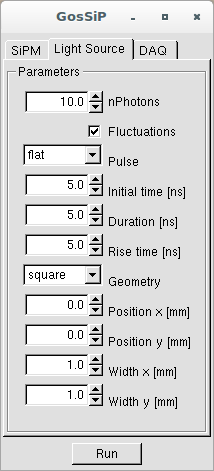
\includegraphics[height=0.25\textheight]{GUI2.png}
\end{figure}

All parameters are members of the daqMC class.

\begin{description}
	\item[Waveform] \textcolor{blue}{\textbf{(Scope())}}\\
		Displays the signal waveform, as measured with an oscilloscope. In addition, the \textit{HitMatrix} is shown: x-axis: pixel number in x, y-axis: pixel number in y, colors: detected photon (blue), dark-count (green), cross-talk (yellow), after-pulse (red).
	\begin{itemize}
		\item \textbf{nEntries} Number of waveforms
		\item \textbf{Integration gate} Measurement time
		\item \textbf{Pregate} Time interval simulated before start of measurement
	\end{itemize}
	\item[Charge Spectrum] \textcolor{blue}{\textbf{(QDCSpectrum(int))}}\\
		Generates the charge spectrum (Single Photon Spectrum).
	\begin{itemize}
		\item \textbf{nEntries} Number of entries
		\item \textbf{Integration gate} Integration gate / measurement time
		\item \textbf{Pregate} Time interval simulated before start of measurement
		\item \textbf{Pedestal} Pedestal value (same units as gain)
	\end{itemize}
	\item[Time Spectrum] \textcolor{blue}{\textbf{(TDCSpectrum(int))}}\\
		Generates the dark-rate time spectrum, i.e.\ the time interval between two consecutive dark-rate pulses.
	\begin{itemize}
		\item \textbf{nEntries} Number of entries
		\item \textbf{Pregate} Time interval simulated before start of measurement
	\end{itemize}
	\item[Threshold Scan] \textcolor{blue}{\textbf{(ThreshScan(double,double,double,double))}}\\
		Generates the dark-rate as a function of the discrimination threshold.
	\begin{itemize}
		\item \textbf{Integration gate} Integration gate / measurement time
		\item \textbf{Pregate} Time interval simulated before start of measurement
		\item \textbf{Threshold start} Start value of discrimination threshold scan
		\item \textbf{Threshold stop} Stop value of discrimination threshold scan
		\item \textbf{Threshold step} Step size of discrimination threshold scan
		\item \textbf{Discri mintime} Minimum time a signal has to be above the threshold to be detected
		\item \textbf{Discri width} Minimum width of the discriminator output pulse
	\end{itemize}
	\item[Statistics] \textcolor{blue}{\textbf{(Statistic(int))}}
		Histogram of the number of fired pixels triggered by photon detection, dark-rate, cross-talk and after-pulsing.
	\begin{itemize}
		\item \textbf{nEntries} Number of entries
		\item \textbf{Integration gate} Integration gate / measurement time
		\item \textbf{Pregate} Time interval simulated before start of measurement
	\end{itemize}
	\item[Response Curve] \textcolor{blue}{\textbf{(DynamicRange(int,double,double))}}\\
		Mean signal charge and RMS as a function of the number of photons. The contribution from different noise sources are indicated by different colours.
	\begin{itemize}
		\item \textbf{nEntries} Number of entries per step
		\item \textbf{Integration gate} Integration gate / measurement time
		\item \textbf{Pregate} Time interval simulated before start of measurement
		\item \textbf{nPhotons max} Maximum number of photons in scan
		\item \textbf{nPhotons step} Step size for the scan
	\end{itemize}
\end{description}


%======= Tutorial (C++) =======%

\chapter{Tutorials (C++)}

\section{Simulate the SiPM Response}

\subsection{Using the LightSource}

\subsection{Building Your Own PhotonList}

\section{Using the DAQ}

\section{Interfacing with Geant4}


\end{document}


